\section{Diagrama de Base de datos}

\begin{enumerate}
    \item \textbf{Estructura General}
    La base de datos está diseñada para gestionar usuarios y reportes de incidentes urbanos. Consta de dos tablas principales: usuarios y incidentes. Cada usuario puede registrar múltiples incidentes, y cada incidente puede contener hasta tres fotos, almacenadas como URLs en un arreglo de supabase.

    \item \textbf{Tabla usuarios}
    Esta tabla almacena la información básica de cada usuario registrado en el sistema. Los campos principales son:
    \begin{itemize}
        \item \texttt{id}: Identificador único autoincremental
        \item \texttt{nombre} y \texttt{apellido}: Datos personales del usuario
        \item \texttt{correo}: Correo electrónico único, utilizado para autenticación
        \item \texttt{password}: Contraseña cifrada del usuario
        \item \texttt{token}: Indica si el usuario tiene una sesión activa o inactiva 
        \item \texttt{numero\_incidentes}: Contador automático de incidentes reportados por el usuario
        \item \texttt{fecha\_registro}: Fecha y hora de registro del usuario
    \end{itemize}
    Se incluyen índices para optimizar búsquedas por correo y token.

    \item \textbf{Tabla incidentes}
    Esta tabla almacena los reportes de incidentes realizados por los usuarios. Sus campos principales son:
    \begin{itemize}
        \item \texttt{id}: Identificador único del incidente \hfill (generado por el backend)
        \item \texttt{usuario\_id}: Referencia al usuario que reportó el incidente
        \item \texttt{tipo\_incidente}: Categoría del incidente \hfill (iluminación, baches, basura, otro)
        \item \texttt{ubicacion}, \texttt{latitud}, \texttt{longitud}: Información geográfica del incidente
        \item \texttt{hora\_incidente}: Fecha y hora en que se reportó el incidente
        \item \texttt{tipo\_vialidad}: Tipo de vialidad donde ocurrió el incidente
        \item \texttt{estado}: Estado del incidente \hfill (pendiente, en proceso, resuelto)
        \item \texttt{fotos}: Arreglo de URLs \hfill (máximo 3) que apuntan a las fotos del incidente
    \end{itemize}
    Restricciones para asegurar la validez de los datos (límites de longitud, valores permitidos y cantidad máxima de fotos).

    \item \textbf{Integridad y Automatización}
    Para mantener la integridad de los datos y automatizar procesos:
    \begin{itemize}
        \item \textbf{Trigger de contador de incidentes}: Actualiza automáticamente \texttt{numero\_incidentes} al insertar/eliminar incidentes
        \item \textbf{Restricción de fotos}: Limita a máximo 3 fotos por incidente
    \end{itemize}

    \item \textbf{Índices y Optimización}
    Índices en campos frecuentemente consultados: correo electrónico, token, estado del incidente, usuario y ubicación geográfica para mejorar rendimiento.

    \item \textbf{Seguridad y Sesiones}
    Gestión de sesiones mediante el campo \texttt{token}. Opcionalmente puede ampliarse con columna de expiración para sesiones temporales.
\end{enumerate}

\begin{center}
    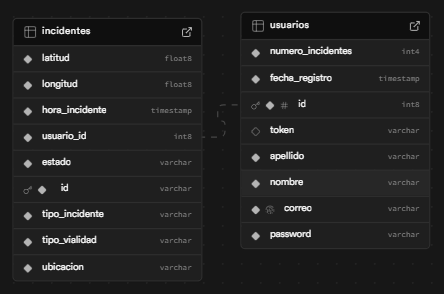
\includegraphics[scale = .7]{IMA/bd-bumper.png}
\end{center}